\documentclass[12pt]{article}
\usepackage{ctex}
\usepackage[english]{babel}
\usepackage{blindtext}
\usepackage{nameref}
\usepackage{fancyhdr}
\usepackage{amsmath,amssymb,amsthm}
\usepackage{graphicx,float}
\usepackage{physics}
\usepackage{pgfplots}
\usepackage[a4paper, total={6in, 9in}]{geometry}

\graphicspath{{../image/}}

\pagestyle{fancy}
\fancyhf{}
\fancyhf[HL]{微分}
\fancyhf[CF]{\thepage}

\newcommand{\innerprod}[2]{\langle{#1},{#2}\rangle}
\newcommand{\id}{\mathtt{id}}

\newtheorem{definition}{定義}
\newtheorem*{theorem}{定理}
\newtheorem*{corollary}{衍理}
\newtheorem*{lemma}{引理}
\newtheorem*{proposition}{設理}
\newtheorem*{remark}{小記}
\newtheorem*{claim}{主張}
\newtheorem*{example}{例子}
\newtheorem*{axiom}{公設}
\renewenvironment*{proof}{\textit{證明.}}{\hfill$\qed$}

\newenvironment*{sol}{\par \textbf{解}.}{\hfill$\blacksquare$}

\begin{document}
    \section*{積分起源}

    討論積分起源,我們依然追溯到牛頓與萊布尼茨的時代。當時牛萊之爭除了微分學的發現以外,還有積分學的建立。雖説兩人整得如火如荼,但我們有著漁翁之利,可以坐享其成。

    但無論如何,之所以存在積分學,是由於一道最基本的問題:假設一物體移動速度$v(t):(0,\infty)\to\mathbb{R}$可以參數$t$量化,則可以下圖表示速度-時間之關係:

    \begin{figure}[H]
        \centering
        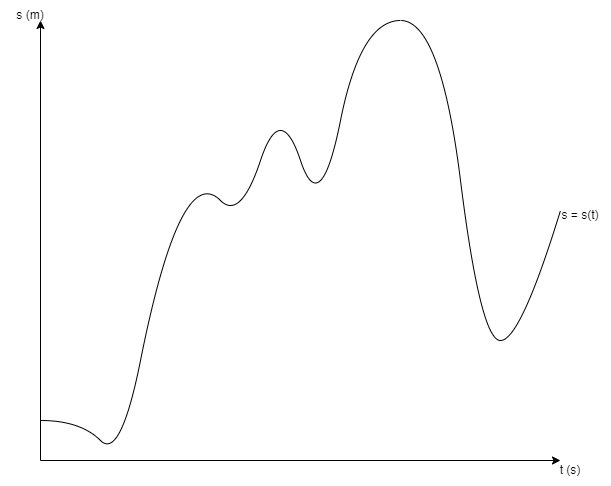
\includegraphics[scale=0.6]{s-t graph.png}
    \end{figure}

    若欲求得任意時間的位移,考慮在極短時間内的瞬間位移相等於瞬時速度乘以時間跨度:設$s(t):(0,\infty)\to\mathbb{R}$為位移函數,則$$\Delta s(t)=v(t)\Delta t$$ 并且總位移應由所有所有瞬間的瞬間位移總和得出,則可考慮將時間均分爲$n$段瞬間,記$t=0$為初始時間及$t_f$為終結時間,并且$0=t_0<t_1<t_2<\cdots<t_n=t_f$,並記對其求和:$$s(t_f)=\sum_{k=0}^{n-1}(s(t_{k+1})-s(t_k))=\sum_{k=0}^{n-1}v(t_k)(t_{k+1}-t_k)$$
    
    \begin{figure}[H]
        \centering
        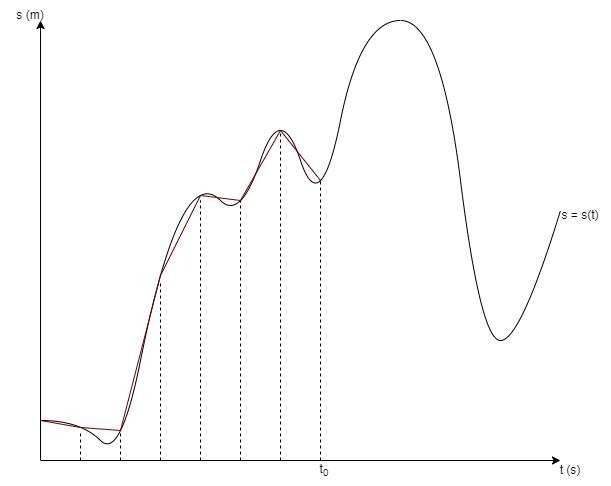
\includegraphics[scale=0.6]{partition s-t.png}
    \end{figure}

    將$n\to\infty$便可定義$$s(t_f)=\int_{0}^{t_f}v(t)dt$$若視$t_f$為變量,則稱其爲\textbf{不定積分};反之,則稱其爲\textbf{定積分}。
    
    \section*{積分的含義}
    從以上簡介可以看出,積分的目的在於加法;更明確的説法是定積分在於計算面積。與中學教程不同,我們會先觀察定積分,再闡述不定積分(實際上他們只差一步)。
\end{document}